\subsection{Data Understanding and Preparation}\label{sec:ts_preparation}
This dataset contains data on the domestic (US and Canada) daily gross income at the box office for 1,134 movies, measured from their release date up to 100 days after release.
The dataset was extracted from Box Office Mojo\footnote{\url{https://www.boxofficemojo.com/}} and contains no missing values, because shorter time series were padded using noise augmented mean.
Each time series was associated with the movie IMDB id, genre and rating (both continuous average rating and a binned version).
In addition to the provided data, we used the IMDB free api\footnote{\url{https://imdbapi.dev/}} to retrieve some additional information about the titles represented in the dataset: title and release year of the movie, runtime (in minutes) number of votes, countries of origin, number of awards and nominations.
We additionally aggregated the box office data as a rough estimate of the total gross income of the movie.

We then splitted our initial dataset reserving 25\% of records for testing and conducted the rest of our analysis exclusively on the training set, as to prevent data leakage.

\subsubsection{Univariate analysis of variables}
The distribution of number of votes, awards, nominations and total gross income show all a pronounced right skew, which is not unexpected. 90\% of records had received awards of nominations.
All records display normal runtimes for movies (between 90 and 200 minutes), except for 3 documentaries which were shorter than 45 minutes.
We were able to detect some outliers also w.r.t. the release year: only two titles were released before 2010 (one in 1969 and one in 1984).

As for the distribution with respect to genres, any given movie can have more than one genre and the most popular genre was \emph{Drama} (48\%), followed by \emph{Comedy} (36\%), \emph{Action} and \emph{Adventure} (each of these 32\%).

We also inspected the distribution of the binned version of rating, finding a considerable unbalance among classes, with \emph{Medium} and \emph{High} being the most frequent ones and the \emph{Low} class representing less than 1\% of titles (cf Fig. \ref{fig:ts_rating_distribution}).

\begin{figure}
    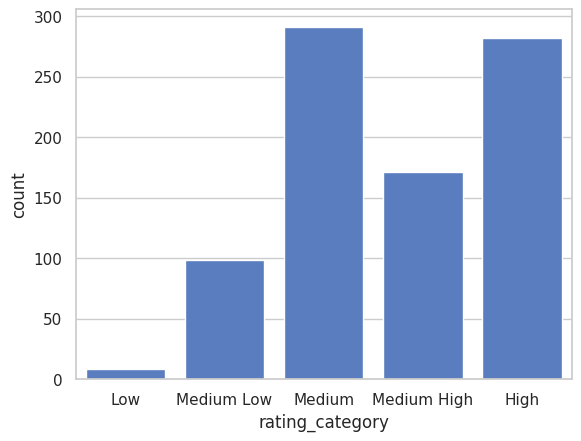
\includegraphics[width=\columnwidth]{../results/images/ts_rating_distribution.png}
    \caption{Distribution of rating category in the Time Series dataset.}\label{fig:ts_rating_distribution}
\end{figure}

\subsubsection{Multivariate analysis of variables}
\begin{figure}[t]
    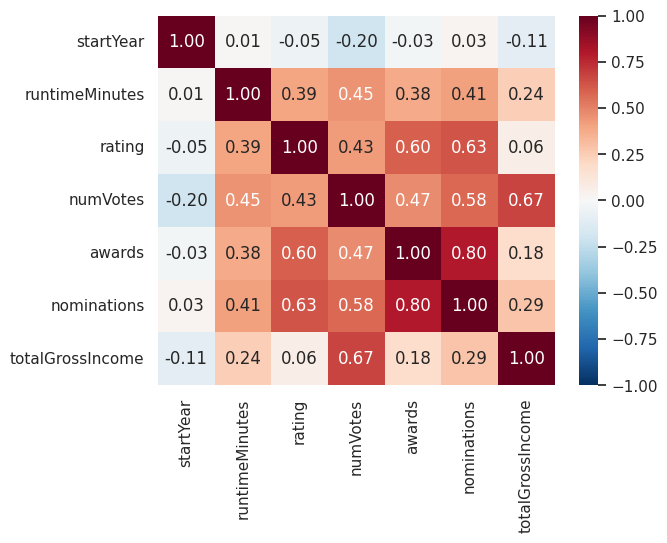
\includegraphics[width=\columnwidth]{../results/images/ts_feat_correlation.png}
    \caption{Correlation of numeric features.}\label{fig:ts_feat_correlation}
\end{figure}

Figure \ref{fig:ts_feat_correlation} reports the Spearman correlation coefficient for pairs of numeric features.
Besides obviously being correlated with each other, both awards and nominations are positively correlated with both the number of votes and rating.
We also observe a moderate to strong positive correlation between the estimated gross income and number of votes.
Perhaps surprisingly, total gross income is only weakly correlated with rating.

Positive correlation of the number votes with rating is something we didn't observe in the IMDB dataset, were, on the contrary these two features were weakly negatively correlated.
We think this may be due to the fact that movies have on average lower ratings than TV Episodes, which, in turn, have fewer votes than movies.
Since the current dataset is limited to movies, we do not observe this (spurious) relationship anymore.

\subsubsection{Visualization}

\begin{figure}
    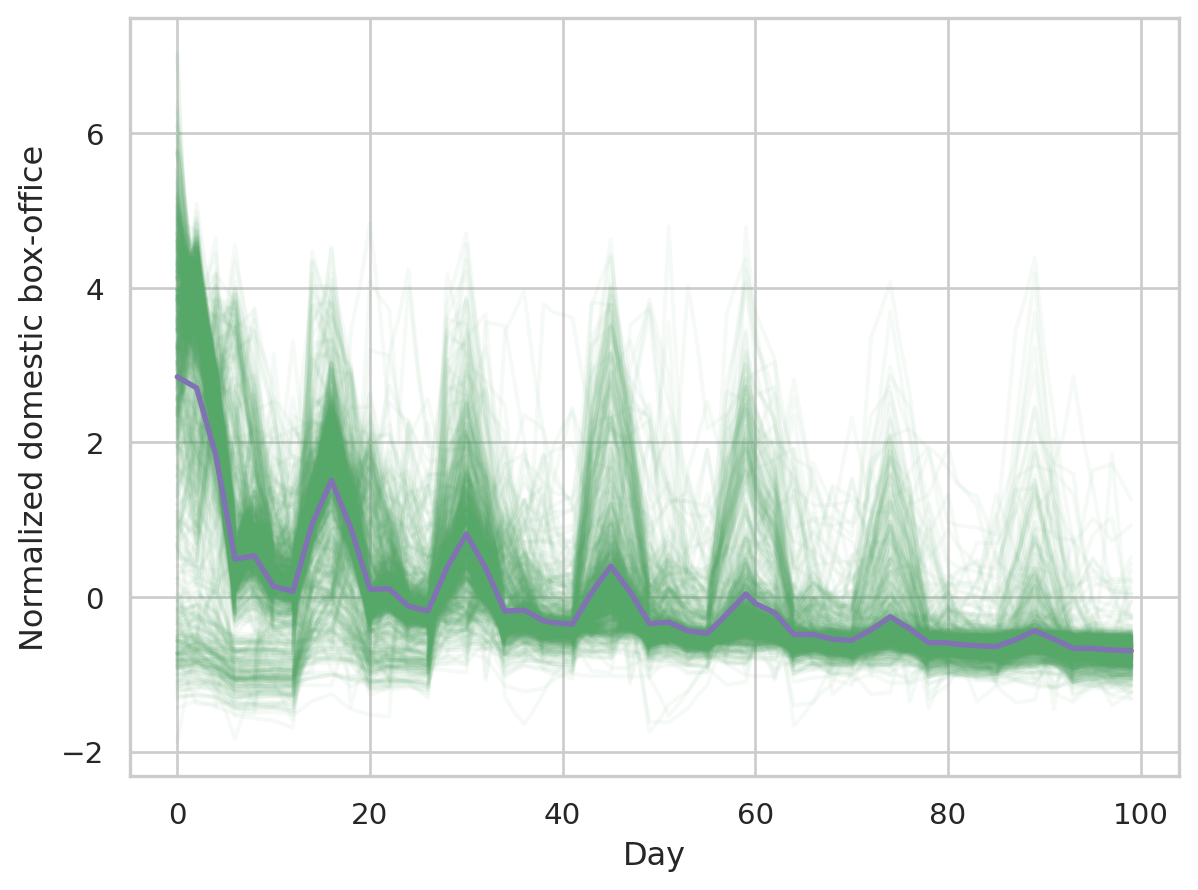
\includegraphics [width=\columnwidth]{../results/images/ts_understanding_viz.png}
    \caption{Time series (and mean time series, in purple) after amplitude scaling}\label{fig:ts_understanding_viz}
\end{figure}

We conclude our understanding visualizing the signals for all time series after amplitude scaling (fig. \ref{fig:ts_understanding_viz}).
Even from this simple visualization we are able to draw some interesting insights.

First of all our time series in general show slightly negative trend and some seasonality with a cycle over around 14 timestamps: this observation was confirmed when we extracted Catch22 features from the time series and were able to verify that most of them had a periodicity of 13 or 14.
This finding, which we initially took at face value, was somewhat puzzling, because we expected a day of week seasonality, with peaks in the weekends, while it made no sense for peaks to occur every other week.
Surely enough, when we finally checked against the original data on Box Office Mojo, we were able to confirm that the observed peaks are, in fact, the effect of day of week seasonality, and that the time series were altered before we received them, either during the extraction or during the preprocessing.

In addition to this discovery, we also were able to observe that, while most movies have profits well over the mean in the first several days after release, some others got a slow start at the box office.
We were able to identify 145 movies that performed below average in the first day of box office. While this is a very coarse distinction, which incurs in some false positives, it was later confirmed by clustering.
In addition to lower box office profits in the first days after release, these `late bloomers' show no clear linear trend (in opposition to the negative trend observed for other movies) and tend to peak on the third weekend after release. We also observed that these were not, for the most part (93\%), action movies.